\documentclass{article}

\usepackage{cheatsheet}

\renewcommand{\sopName}{ACS}
\renewcommand{\sopVersion}{02-OCT-2016}
\renewcommand{\sopEditor}{(cwe)}


\begin{document}
\sopHeadSkip%

\vfill

\notes{%
  \begin{itemize}
    \item \textbf{CAVE:} \hspace{1mm} DD Aortenaneurysma
    \item {\Ox} nur bei {\SpOx} < \SI{94}{\percent} oder Dyspnoe
    \item Aspirin auch bei Dauermedikation
    \item Diagnose-to-Balloon {\zeit} < \SI{90}{\minute}
  \end{itemize}
}

\vfill

\drug{Nitrolingual {\small(Glyceroltrinitrat)}}{%
  \dosierung{\SI{1}{\hub} (\wdh{1} | \SIrange{3}{5}{\minute})}
  \begin{kontraindikationen}
    \item \textbf{RR} < \SI{110}{\mmHg}
    \item bekannte Rechtsherzbelastung bei COPD
    \item diagnostizierter Rechtsherzinfarkt
    \item Einnahme PDE-5-Hemmer
      (Viagra {\uhr} < \SI{24}{\hour} | Cialis {\uhr} < \SI{36}{\hour})
  \end{kontraindikationen}
}

\vfill

\drug{Aspirin {\small(Acetylsalicylsäure)}}{%
  \dosierung{\SI{250}{\milli\gram} i.v.}
  \begin{kontraindikationen}
    \item Asthma / COPD
    \item Ulcus, GI-Blutung, Teerstuhl, Bluterbrechen
  \end{kontraindikationen}
}

\vfill

\drug{Heparin {\small(Heparin-Natrium)}}{%
  \dosierung{\SI{60}{\IE\per\kgKG} (\SI{5000}{\IE}) i.v.}
  \begin{kontraindikationen}
    \item Heparin induzierte Thrombozythopenie
    \item Therapierefraktäre Hypertonie
    \item Frische Blutung, GI-Blutung, Teerstuhl
    \item OP/arterielle Punktion {\zeit} < \SI{7}{\day}
    \item bösartiger Tumor
  \end{kontraindikationen}
}

\vfill

\notes{%
  \begin{center}
    \hspace{-2.5em}
    \rotatebox{90}{%
      \fontsize{16pt}{16pt}\selectfont\color{myBlue}
      \hspace{2mm}EKG Beispiel
    }
    \hspace{1em}
    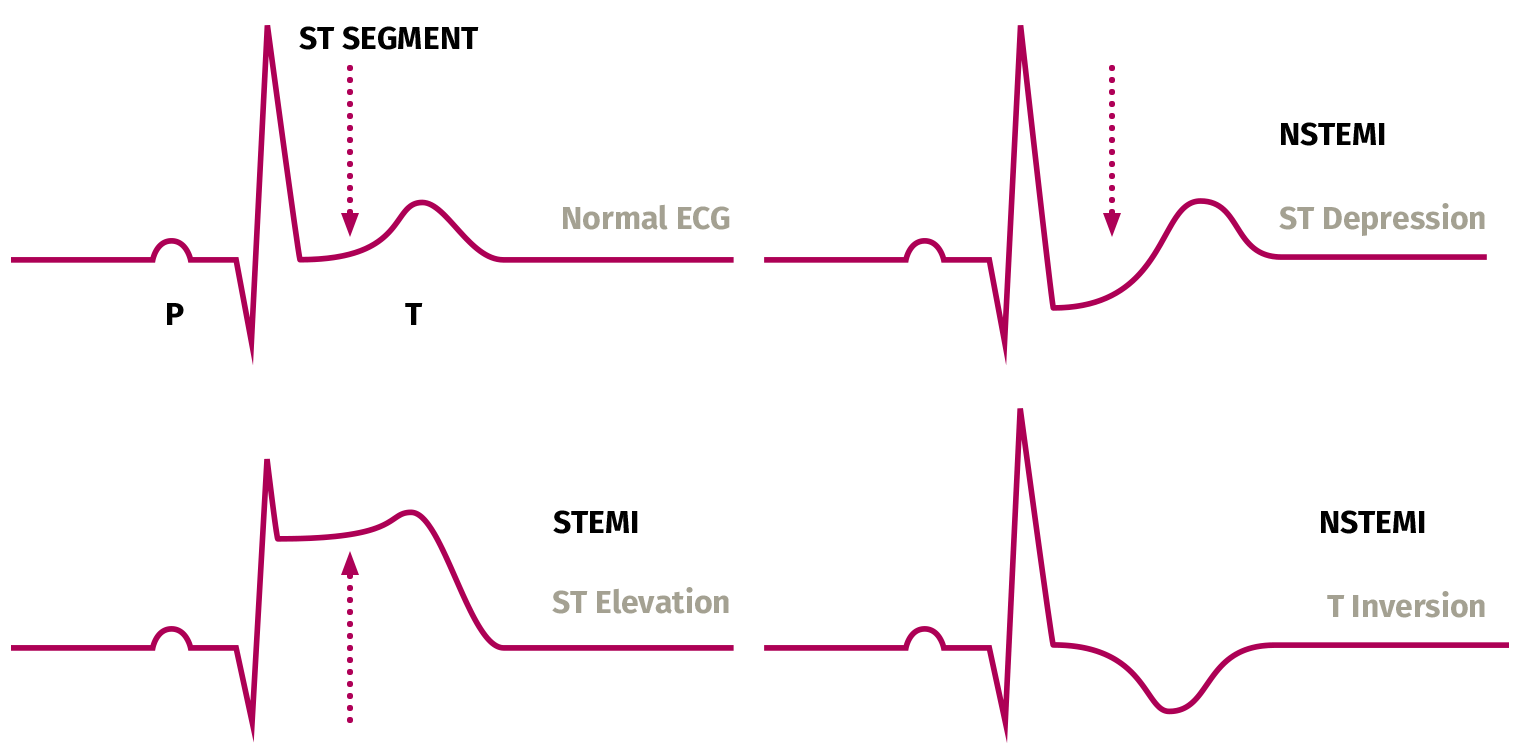
\includegraphics[width=0.75\textwidth]{img/stemi.png}
  \end{center}
}

\vfill

\end{document}
